\documentclass{beamer}
\usetheme{metropolis}

\usepackage[utf8]{inputenc}
\usepackage[normalem]{ulem}
\usepackage{csquotes}

\title{IDU1321. Ettevõtte äriarhitektuur}
\subtitle{Teine loeng}
%\date{10.09.2017}
\author{Andres Kütt}
\institute{Cybernetica, arhitekt}


\begin{document}

\begin{frame}
\titlepage
\end{frame}

\section{Modelleerimine}

\begin{frame}[standout]
Küsimusi loetu kohta?
\end{frame}

\section{Kommunikatsioon}
\begin{frame}{Kommunikatsiooni põhimudel}
\begin{center}
	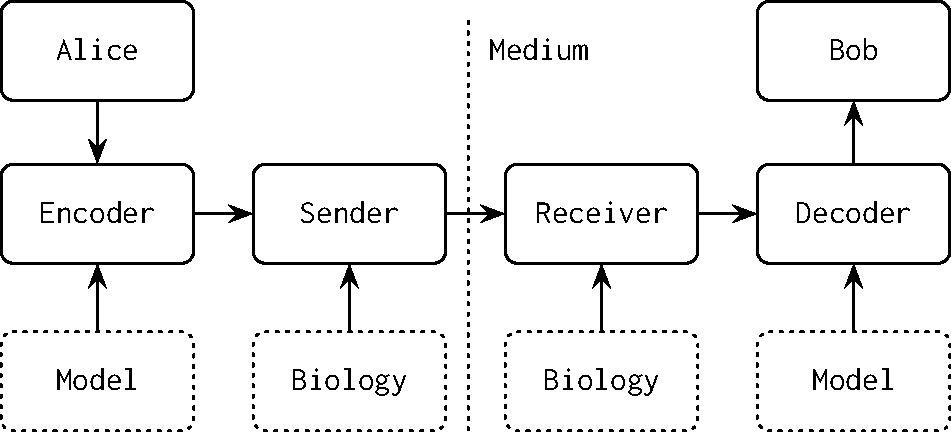
\includegraphics[width=.8\textwidth]{communication_model.pdf}
	\end{center}
\end{frame}

\begin{frame}{Mudeli järelmid}
	\begin{itemize}
		\item Igal sammul informatsioon muutub
		\begin{itemize}
			\item Bioloogilised faktorid
			\item Kultuurilised faktorid
			\item Keskkonnafaktorid
		\end{itemize}
		\item Kanalis on alati müra
		\item Mõlemad osapooled opereerivad alati (erinevas) kontekstis
		\item Kommunikatsiooniakt sisaldab alati tagasisidet
		\begin{itemize}
			\item Sest me alustame suhtlemist põhjusega
			\item Ka tagasiside tuleb läbi nendesamade kihtide
		\end{itemize}
	\end{itemize}
\end{frame}

\begin{frame}[fragile]
	\begin{center}
		\LARGE{\textbf{Edukaks kommunikatsiooniks on kriitiline hoiduda müra kuhjumisest}}
		\\[4cm]
		\small{Alati kontrolli, kuidas sinust aru saadi}
	\end{center}
\end{frame}


\section{Mudelitest}
\begin{frame}[fragile]
	\begin{center}
		\LARGE{\textbf{Kõik mudelid on valed, \\mõned mudelid on kasulikud}}
		\\[4cm]
		\small{Iga mudel on definitsiooni järgi lihtsustus lõputult keerulisest maailmast.\\Kuidas mu mudel kasulik on ja kellele?}
	\end{center}
\end{frame}

\begin{frame}{Miks joonistada mudeleid?}
\begin{description}
	\item[Kommunikatsioon] Mudel kui viis suhelda, toimetada mõte minu peast kellegi teise pähe
	\item[Mõtlemise vahend] Mudel kui viis mõelda, kui viis kontrollida oma mõtte konsistentsust
	\item[Süsteemi formaalne kirjeldus] Mudel kui andmestik, kui viis süsteemi kohta rangeid väiteid esitada
\end{description}
	
\end{frame}

\begin{frame}{Mudeldamise peamised ohud}
	\begin{itemize}
		\item Mudel muutub asjaks iseensest
		\item Aetakse segi mudel ja reaalsus
		\item Eeldatakse täiuslikku kommunikatsiooni
		\item Kuritarvitatakse mudeli(tarkvara) võimalusi
		\item Loovuse kadu
	\end{itemize}
\end{frame}

\section{Üldist mudelitest}

\begin{frame}{Mida me mudeldame}
	\begin{itemize}
		\item Objektid
		\begin{itemize}
			\item Miski, millel on stabiilne eksistents mingiks ajaks
			\item Neil võib olla olek
			\item Moodustavad süsteemi vormi
		\end{itemize}
		\item Protsessid
		\begin{itemize}
			\item Miski, mis rakendub ühele või mitmele objektile
			\item Võib muuta objektide olekut
			\item Leiab aset ajas
		\end{itemize}
	\end{itemize}
\end{frame}

\begin{frame}{Seosed}
	\begin{itemize}
		\item Formaalsed seosed
		\begin{itemize}
			\item Seosed, mis eksisteerivad (või võivad eksisteerida) stabiilselt mingi aja jooksul
			\item Asjad on teiste asjade kõrval/peal/küljes
		\end{itemize}
		\item Funktsionaalsed seosed
		\begin{itemize}
			\item Seosed, mis teevad midagi
			\item Midagi muudetakse, liigutatakse või vahetatakse
			\item Mõnikord kutsutakse interaktsioonideks
		\end{itemize}
	\end{itemize}
	
	\begin{center}
		\textbf{Tüüpiliselt funktsionaalne seos eeldab formaalset seost, vastupidine ei ole tõsi}
	\end{center}
\end{frame}

\section{Harjutus}

\begin{frame}{Kohvitass}

\begin{itemize}
	\item Miks me modelleerimie?
	\item Mida \emph{kasulikku} see asi teeb?
	\item Millistest tükkidest ta koosneb?
	\item Millised on seosed tükkide ja funktsiooni vahel?
\end{itemize}

\end{frame}

\begin{frame}{ERP}

\begin{itemize}
	\item Miks me modelleerimie?
	\item Mida \emph{kasulikku} see asi teeb?
	\item Millistest tükkidest ta koosneb?
	\item Millised on seosed tükkide ja funktsiooni vahel?
\end{itemize}

\end{frame}


\begin{frame}{Harjutuse kokkuvõte}
	\begin{itemize}
		\item Kas teie arusaam süsteemist paranes?
		\item Kuidas erines füüsilise ja tarkvaralise süsteemi modelleerimine?
		\item Kumma puhul on eri liiki seoste eristamine lihtsam?
	\end{itemize}
\end{frame}

\begin{frame}{Kordame}
	\begin{itemize}
		\item Kommunikatsioon
		\item Mudelitest
		\item Mudeldamise ohud
		\item Objektid/protsessid
	\end{itemize}
\end{frame}

\begin{frame}{Järgmine kord}
\begin{itemize}
	\item Strateegia
	\item Juht kui disainer
	\item Kuidas organisatsioonid käituvad?
	\end{itemize}
\end{frame}

\begin{frame}[standout]
Küsimusi?
\end{frame}

\end{document}
